\section{Integrerade Kretsar (IC)}

\subsection{Allmänt om IC}
\index{integrerad krets}
\index{IC}

Att integrera betyder att samla till en enhet, det kan vara komponenter,
funktioner, verksamheter etc. Integration kan ske på olika nivåer och i många
olika sammanhang.

Med integration avses här komponenter för elektroniska strömkretsar. Särskilt
halvledarelement av olika slag samt resistorer och kondensatorer med små värden
kan framställas med små dimensioner. Många komponenter kan då samlas i samma
hölje.

Komponenter inom ett hölje, avsedda för en viss funktion kallas
\emph{integrerad krets} (eng. \emph{Integrated Circuit -- IC}).

Komponenterna i en IC kan i sin tur vara del av komponenterna en hel strömkrets.
Redan inom höljet kan komponenter kopplas samman för en viss funktion eller som
en del av strömkretsen. Skrymmande eller effektkrävande komponenter, såsom
induktorer, transformatorer osv. får emellertid inte plats, varför även yttre
kopplingar behövs. Det kan också behövas flera IC i en strömkrets -- kanske med
innehåll för en annan funktion.

\subsection{Integrationsgrad}

En integrerad krets är uppbyggd på en basplatta av halvledarmaterial --
ett chip.
På plattan framställs, med fototeknik eller etsning, kompletta eller nästan
kompletta dioder, transistorer, resistorer och kondensatorer. Metoden, som
kallas planarteknik, medger att många komponenter kan få plats på samma platta.

Den snabba utvecklingen av produktionsmetoder för integrerade kretsar gör
alltmer avancerade system möjliga och dessutom på allt mindre utrymme. Med
avseende på integrationsgrad används följande begrepp.

\begin{tabular}{lp{6cm}}
SSI & Small Scale Integration innebär något 10-tal halvledare på samma chip. \\
MSI & Medium Scale Integration innebär något 100-tal halvledare på ett chip. \\
LSI & Large Scale integration innebär något 10000-tal halvledare på ett chip. \\
VLSI & Very Large Scale Integration innebär 100000 eller fler halvledare. \\
\end{tabular}

\subsection{Olika slags integrerade kretsar}

Det finns stora sortiment av både standardiserade och speciella IC, varav det
finns två huvudtyper:
\begin{itemize}
  \item digitala integrerade kretsar
  \item analoga integrerade kretsar.
\end{itemize}

\subsection{Digitala IC}

Digitala IC arbetar som framgår av namnet med digitala signalnivåer. De enklaste
typerna innehåller en eller flera digitala grindar (se avsnitt
\ref{digitala kretsar}).
Genom att koppla samman grindar kan man skapa kretsar för ett visst ändamål.
I början av 70-talet byggdes komplicerade system av grindar i SSI- och
MSI-teknik.
Ett sådant system är emellertid inte flexibelt eftersom eventuella ändringar
måste göras ''hårdvarumässigt''.
Det innebär att kopplingsledningar måste ändras om, kanske hela kretsar bytas
ut osv.

I dagens digitala system används IC i form av en mikroprocessor eller till och
med flera.
En mikroprocessor är en avancerad LSI-krets, som kan programmeras
(kopplas upp) ''mjukvarumässigt'' inte bara för ett ändamål utan för många
olika. I system med mikroprocessorer behövs också minnesfunktioner. Sådana kan
också samlas i LSI-kretsar. Mikroprocessorn är hjärtat i en dator. Styrd av ett
program (mjukvaran) styr den kringutrustningar med uppgift att inhämta och avge
information -- att kommunicera.

\subsection{Analoga IC}

Analoga IC arbetar med analoga signalnivåer, dvs. spänningar och strömmar med
många olika nivåer och frekvenser. En analog IC kan därför även arbeta med
digitala signaler.

Analoga IC innehåller en balanserad förstärkare eller flera samt olika slags
hjälpkretsar. Med yttre komponenter kan en analog IC ges olika förstärkning och
frekvensgång. Gemensamt namn för dessa förstärkare är operationsförstärkare
(OP-amp). OP-förstärkare utförs vanligen i SSI- eller möjligen MSI-teknik.

\subsection{Kombinerade och speciella IC}

Utöver standardiserade IC finns kombinerade och speciella IC.

Exempel på speciella digitala IC är sådana för telekommunikationsändamål.

Ett annat exempel på digitala IC är sådana för signalbehandling, såväl på HF som
LF-nivå.

Exempel på speciella analoga IC är sådana för radiokommunikationsändamål.

Bortsett från vissa skrymmande komponenter och manöverdonen kan numera till exempel en
IC innehålla en komplett radiomottagare. Ett annat exempel på speciella analoga
IC är sådana för hörapparater. Genom programmering anpassas de för det
personliga behovet.

\subsection{Utvecklingen}

Det kan sägas hur ofta som helst. Genom den fantastiska utvecklingen av
mikroelektronik öppnas även för radioamatören möjligheter, som bara för ett par
decennier inte var tänkbart.

Denna utveckling har vidgat utrymmet för den experimentella verksamhet som
amatörradio i grunden innebär. Hobbyn får sålunda med tiden en allt större
teknisk spännvidd.

\subsection{Aktuell litteratur}

Ökat teknikomfång inom amatörradio ställer motsvarande krav på litteratur. På
senare tid inbegripes även digitalteknik. Mest av utrymmesskäl behandlas i denna
faktabok digitaltekniken mycket kortfattat, men ändå så mycket som nämns i
CEPT-rekommendationen T/R 61-02. För djupare studium hänvisas till andra
läromedel samt till leverantörskataloger.

\section{Operationsförstärkare}
\textbf{
HAREC a.\ref{HAREC.a.2.8.3}\label{myHAREC.a.2.8.3}
}
\index{operationsförstärkare}
\index{op-amp}

\emph{Operationsförstärkare} (eng. \emph{operational amplifier}), ofta kallad
för \emph{op-amp} är en integrerad kretstyp som har hög förstärkning.
Istället för att ha enbart en ingång så har den två, en positiv
och en negativ, och operationsförstärkaren förstärker skillnaden mellan den
positiva och negativa signalen. Förstärkningen i en modern operationsförstärkare
kan vara i storleksordningen med en miljon.
De två mest grundläggande kopplingarna man använder är komparator respektive
negativt återkopplad förstärkare.

\subsection{Komparator}

I en \emph{komparator} används den höga förstärkningen för att få även små
spänningsskillnader att ger stort utslag. Med referens-spänningen på den
negativa ingången och insignalen på den positiva ingången så kommer utgången
att vara så hög den kan vara när ingången har högre spänning än
referensspänningen, och omvänt kommer den vara så låg den kan vara när ingången
är lägre än referensspänningen.

Det är enkelt att få utgången att ha omvänd egenskap, genom att växla signaler
mellan positiv och negativ ingång på operationsförstärkaren.

\subsection{Negativ återkoppling och förstärkare}

En operationsförstärkare som har en negativ återkoppling, dvs. där signal från
utgången matas tillbaka till den negativa ingången, får den egenskapen att den
försöker driva utgången så att spänningarna för den positiva och negativa
ingången blir densamma.
Det finns en rik uppsättning kopplingar som bygger på denna jämvikt, där
operationsförstärkaren opererar i en linjär förstärkningsmod.

Denna jämvikt gör också att en snabb diagnosticering kan göras genom att mäta
spänningen mellan ingångarna, är den i princip noll så fungerar kopplingen
förmodligen, medan har den gått sönder på något sätt, till exempel trasig op-amp
eller trasig återkoppling så kommer spänningen vara synbart annorlunda och
jämvikten finns inte.

\subsubsection{Bufferförstärkare}

Den enklaste linjära kopplingen med en operationsförstärkare är en
bufferförstärkare.
I denna koppling är den negativa ingången direkt kopplad till utgången
samt insignalen till den positiva ingången.
Med denna koppling kommer op-ampen försöka få den negativa ingången och direkt
därmed utgången att följa insignalen.
Det gör att man i den ideala av världar har samma spänning ut som man har in,
vilket även kallas för spänningsföljare.
Fördelen är att lasten på utgången kan vara oerhört mycket högre, och
om utgången skulle sjunka beroende på lasten försöker återkopplingen driva den
till rätt spänning.

Bufferförstärkaren gör att OP-ampen kan leverera samma spänning ut men mot en
last på fåtal ohm, dvs. med mycket större strömstyrka.
Den relativt höga ingångsimpedansen hos op-ampen, upp mot en teraohm, gör att detta
kan ske utan större påverkan på ingångskretsen.

\subsubsection{Positiv, icke-inverterande, förstärkning med op-amp}
\label{icke-inverterande förstärkning}

En enkel variant på bufferförstärkaren är att man kopplar in en spänningsdelare
mellan utgången och den negativa ingången, så som illustreras i bild
\ref{fig:BildII2-46}.

\begin{wrapfigure}{R}{0.5\textwidth}
	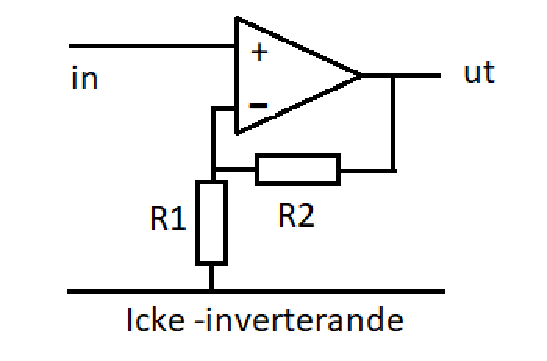
\includegraphics[width=0.5\textwidth]{images/cropped_pdfs/bild_2_2-46.pdf}
	\caption{Icke-inverterande förstärkare}
	\label{fig:BildII2-46}
\end{wrapfigure}

Om spänningsdelaren är till 1/10 så kommer alltså utgången behöva öka 10 gånger
mer än den negativa ingången förändrar sig, och op-ampen kommer därför driva
utgången 10 gånger den positiva ingången, för att lyckas hålla balansen.
På detta sätt kan man sätta förstärkningen hos förstärkaren.
Förstärkningen blir:

\(G = 1+ \dfrac{R_2}{R_1}\)

Genom att sätta en kondensator parallellt med motståndet som går mellan utgång
och den negativa ingången kan man skapa en bandbreddsbegränsning för
förstärkaren.
För de högre frekvenserna kommer merparten av strömmen att gå genom
kondensatorn och motkopplingen blir därför högre än för låga frekvenser.
Förstärkningen för höga frekvenser sänks ned mot nivån för en bufferförstärkare.

Detta är också ett sätt att försäkra sig om att kretsen inte självsvänger vid
höga frekvenser.

\subsubsection{Negativ, inverterande, förstärkning med op-amp}
\label{inverterande förstärkning}
\label{virtuell jord}
\label{jordning!virtuell}

Om man som i bild \ref{fig:BildII2-47} istället för positiv förstärkning vill
ha negativ förstärkning så tar man och ansluter den positiva ingången till jord
och spänningsdelaren på den negativa ingångens sida kopplar man loss från jord
och ansluter till insignalen.

\begin{wrapfigure}{R}{0.5\textwidth}
	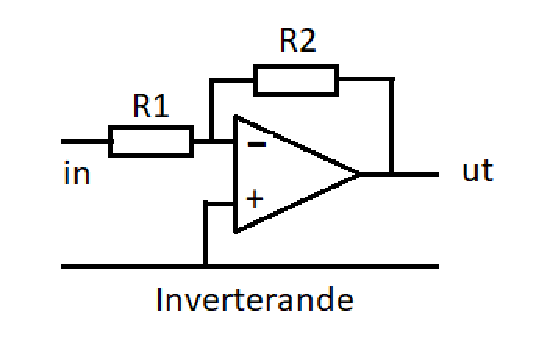
\includegraphics[width=0.5\textwidth]{images/cropped_pdfs/bild_2_2-47.pdf}
	\caption{Inverterande förstärkare}
	\label{fig:BildII2-47}
\end{wrapfigure}

Nu kommer op-ampen att balansera den negativa ingången så att den är på samma
potential som jord, detta kallas för \emph{virtuell jord}.
Strömmen kommer gå från ingången till utgången, men ingången kommer se lasten
av ingångsmotståndet \(R_1\) och utgången kommer mata \(R_2\) mot jord.
Förstärkningen kommer vara negativ och proportionell mot motståndens inbördes
relation, dvs.:

\(G = -\dfrac{R_2}{R_1}\)
